\subsection{Beam Quality(Purity)}

We have several beam counters to indentify beam particles event by event(see Fig\ref{fig:Beamline}).Using this when taking data, we can get data of interest selectively.The following describe how to identify beam particles with the typical data including $K^{+}$, $\pi~{+}$, $e^{+}$, $p$ events, which have the momentum adjusted $\sim$800MeV/c.\\

\begin{figure}[htbp]
  \centering
  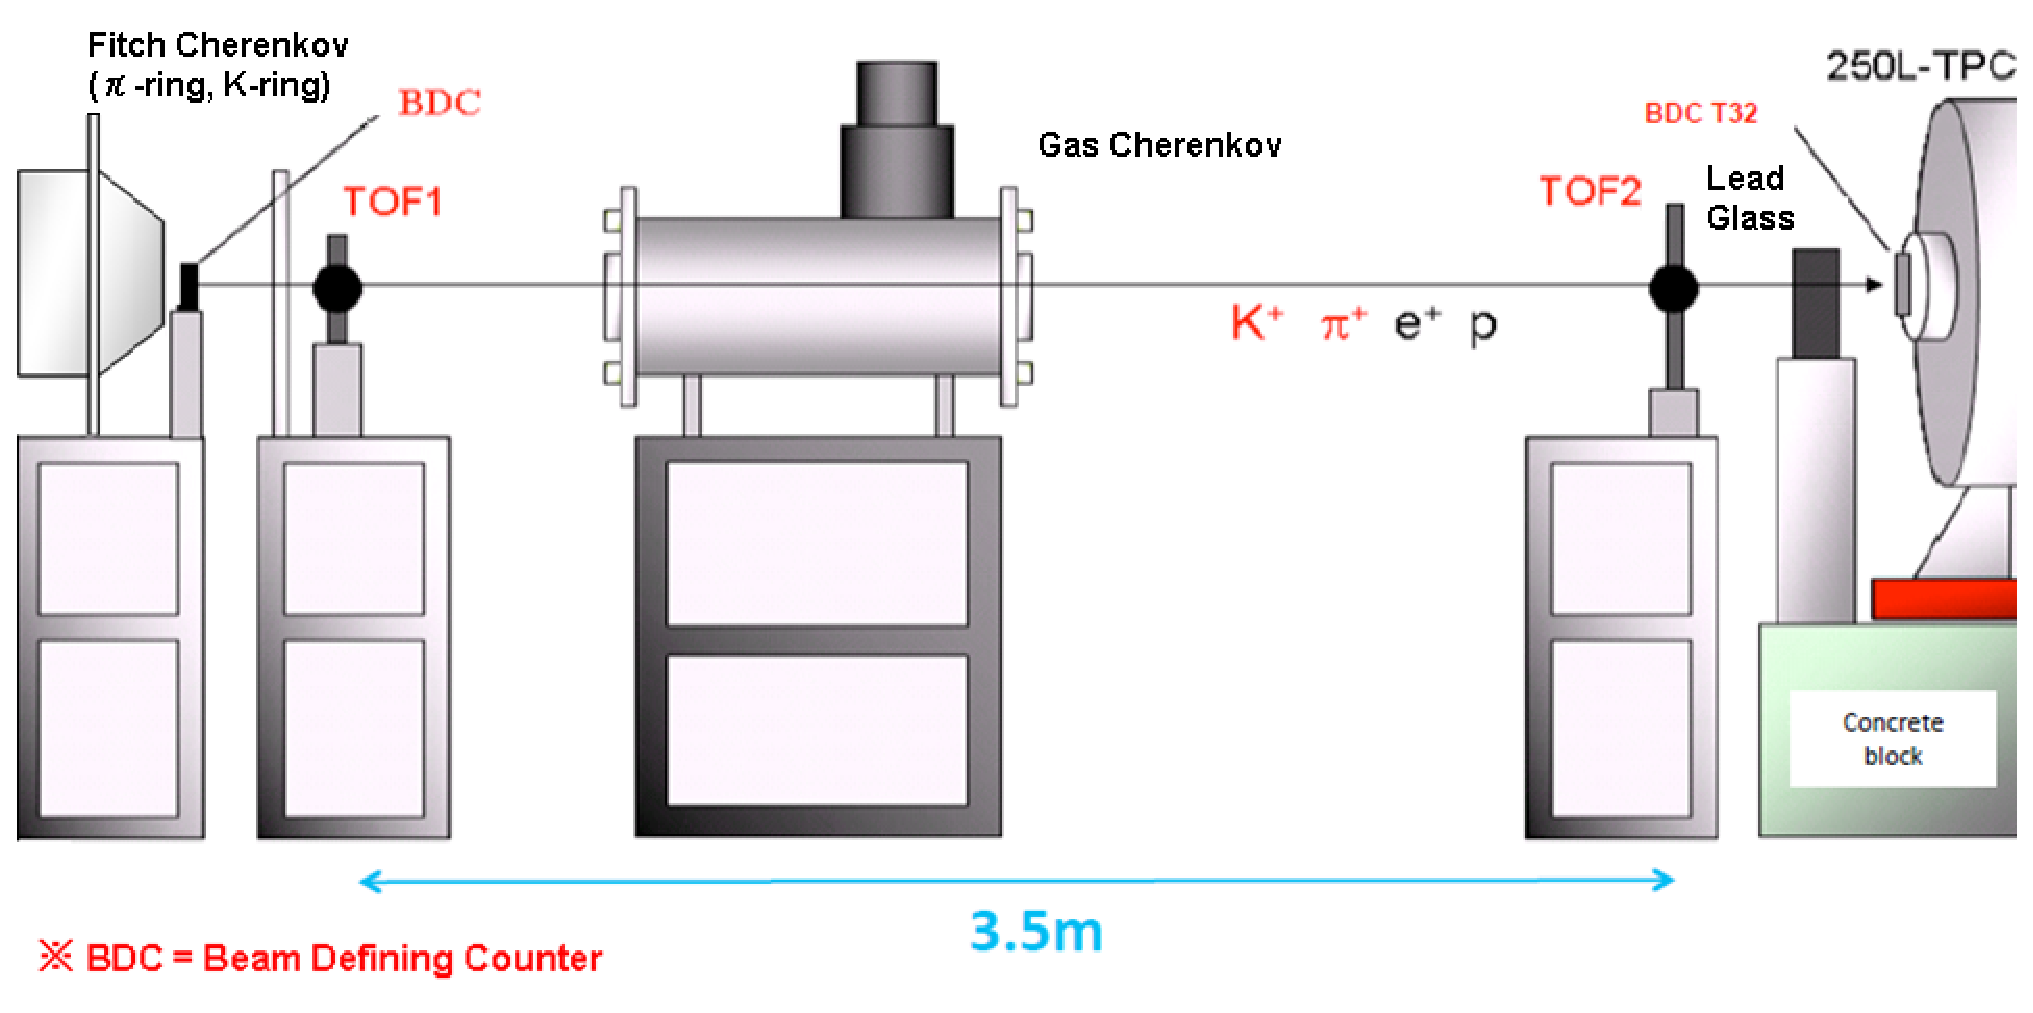
\includegraphics[width=10cm,clip]{fig/Beamline.eps}
  \caption{Instruments on K1.1BR Beam Line}
  \label{fig:Beamline}
\end{figure}

Leaded particles to K1.1BR beamline pass the Fitch Cheernkov Counter at first.
Fitch Cherenkov Counter can select particles with diffrerences of angle of cherenkov light which they radiate.
Fifure\ref{fig:FC_KPI} shows the respose of the Fitch Cherenkov Counter.
The horizontal axis shows the total amount of PMT signal where cherenkov light of 800MeV/c $\pi$ can be detected.
The vertical axis shows that of 800MeV/c $K$.
Signals are distinctly seperated to three cluster and can be categolized as following.\\

\begin{enumerate}
\item FC($\pi$) Signal$<$1450 \& FC($K$) Signal$>$2000 \\
\item FC($\pi$) Signal$<$1450 \& FC($K$) Signal$<$2000 \\
\item FC($\pi$) Signal$>$1450 \& FC($K$) Signal$<$2000 \\
\end{enumerate}

Appearently, particles within the region 1 are $K^{+}$ candidates.
Particles within region 2 are $p$ candidates because 800MeV/c $p$ is impossible to radiate cherenkov light.
Particles within region 3 are $\pi^{+}$ or $e^{+}$ candidates because their angle of cherenkov light are almost same level.\\

\begin{figure}[htbp]
  \centering
  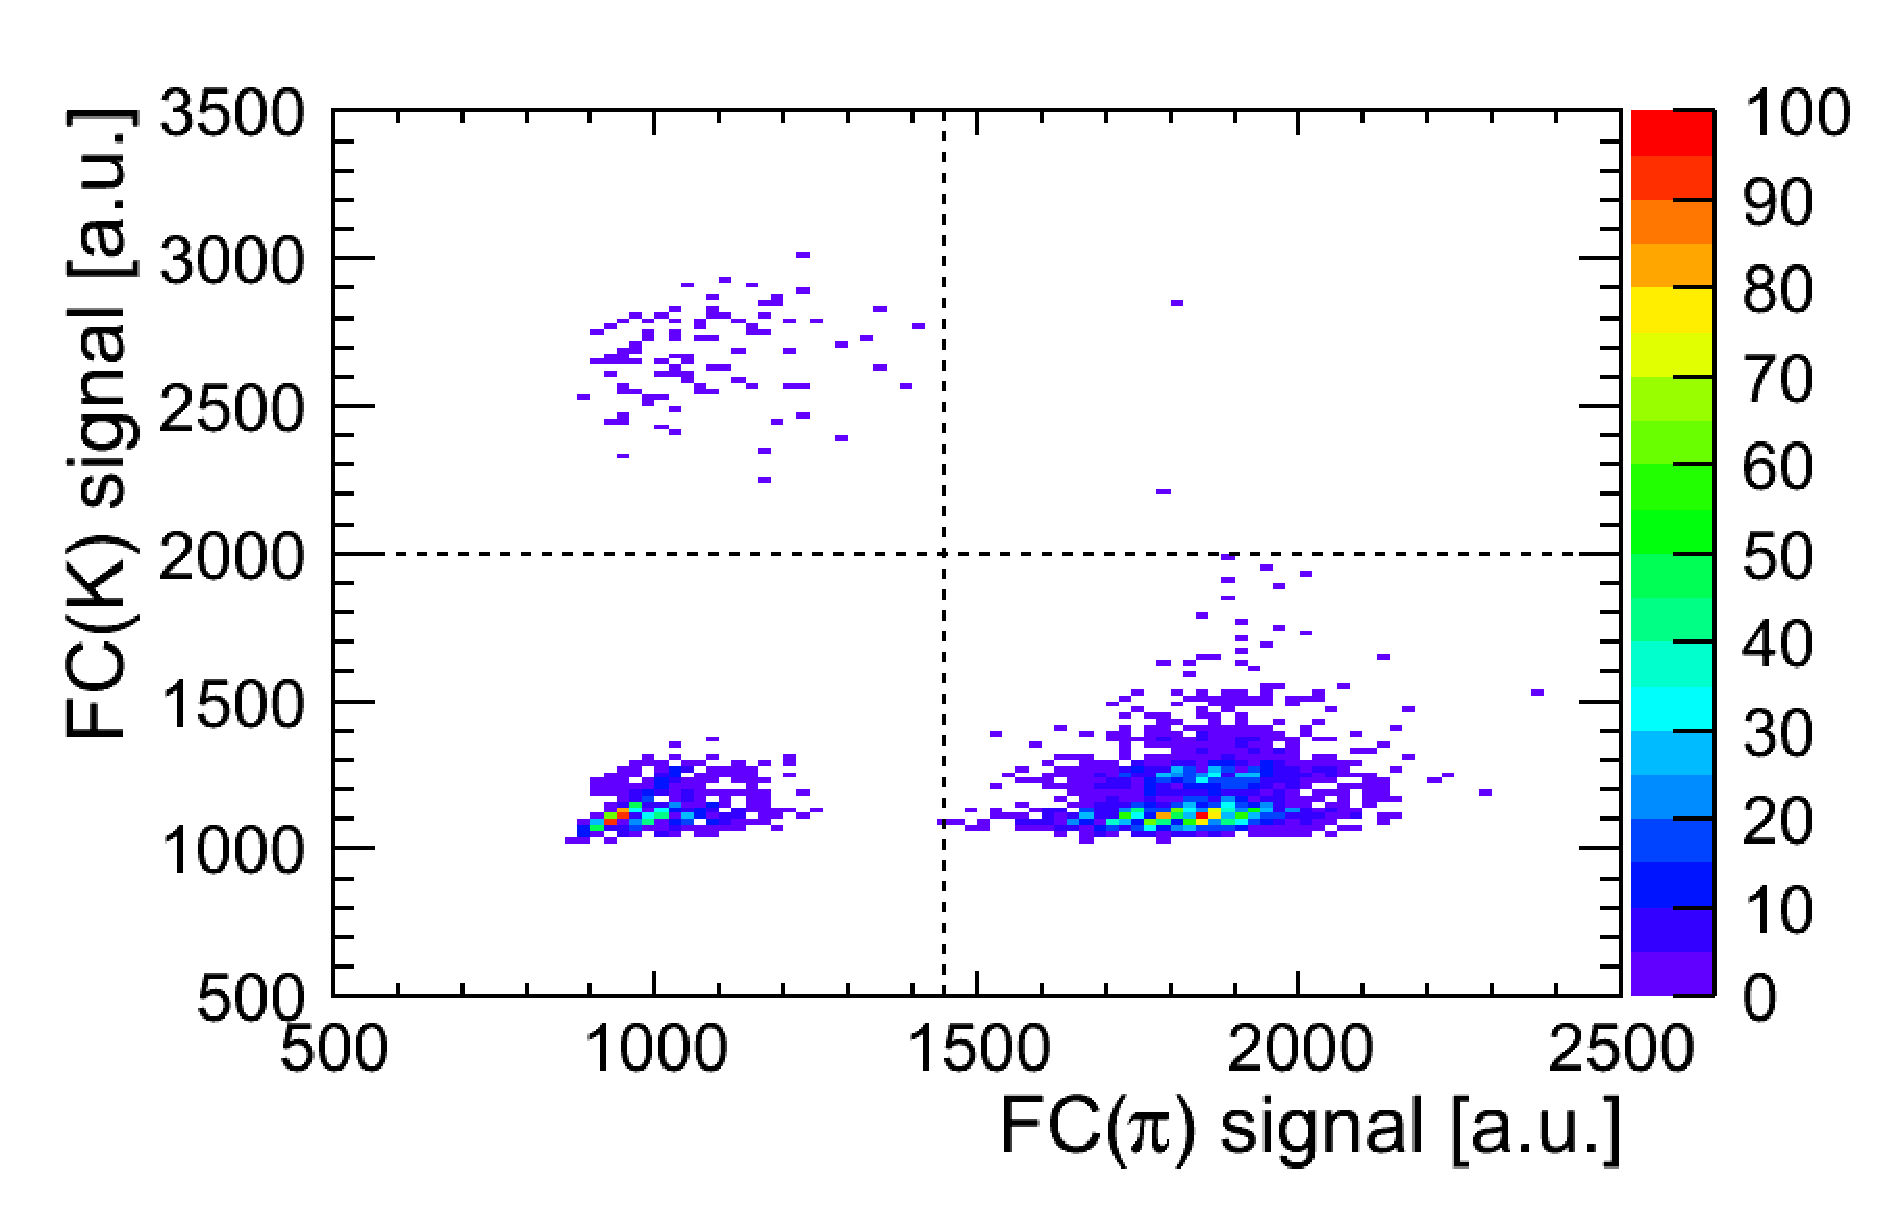
\includegraphics[width=10cm,clip]{fig/FC_KPI.eps}
  \caption{Fitch Cherenkov Counter}
  \label{fig:FC_KPI}
\end{figure}

Gas Cherenkov Counter can select $e^{+}$ from the other particles because only $e~{+}$ can radiate cherenkov light at the refractive index of this gas.
Figure\ref{fig:GC} shows the responce of the Gas Cherenkov Counter.
The horizontal axis shows the PMT signal of the Gas Cherenkov Counter.
The vertical axis shows the number of events.
Fitting the pedestal with gaussian function,
the events larger than the value added $\sim$3.5$\sigma$ to the mean of the pedestal is $e^{+}$ candidates.In this case, GC signal is required more than 104.7 to be $e^{+}$ candidates.\\

\begin{figure}[htbp]
  \centering
  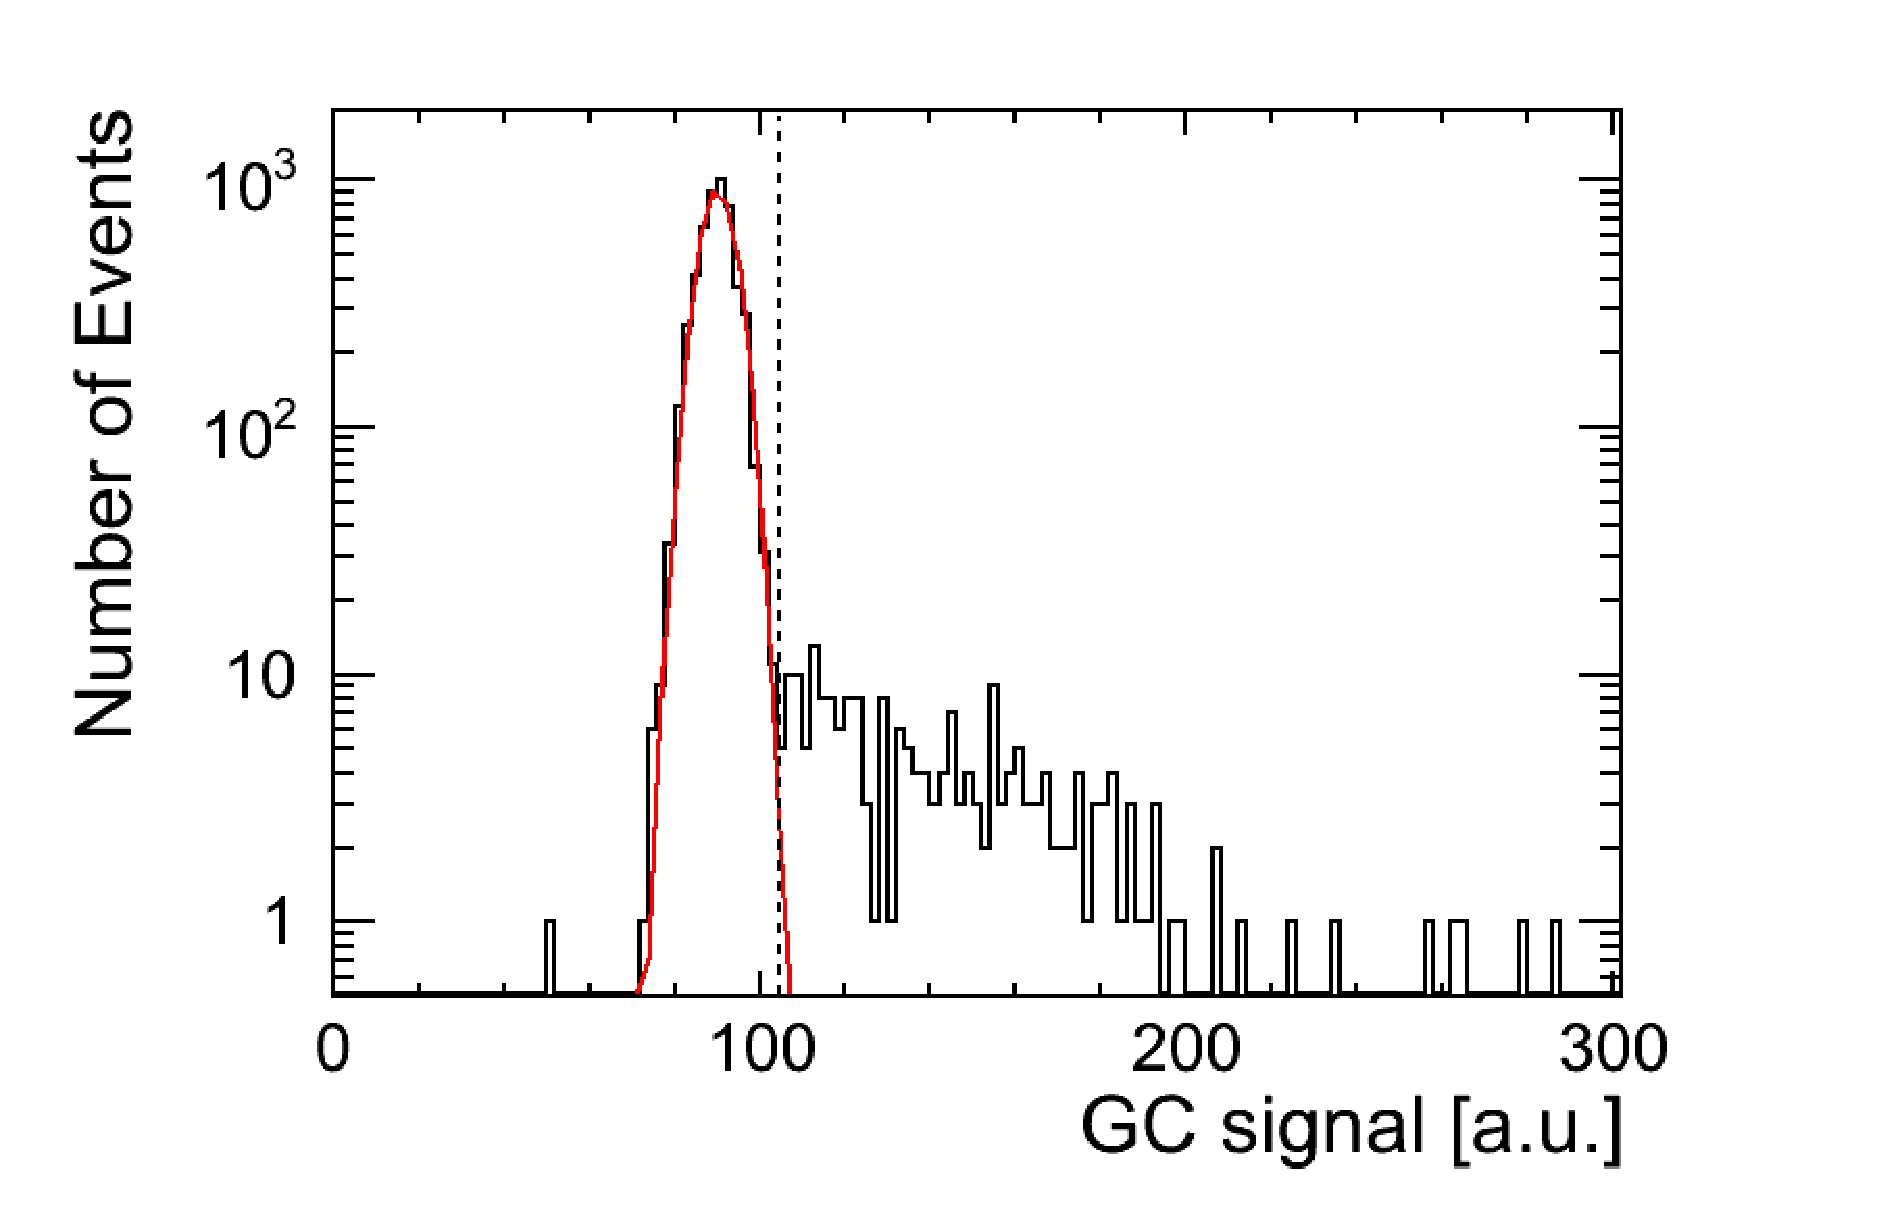
\includegraphics[width=10cm,clip]{fig/GC.eps}
  \caption{Gas Cherenkov Counter}
  \label{fig:GC}
\end{figure}

There are two TOF Counters which has $\sim$200ps resolution 3.5m apart, 
and each particle can be selected with the difference of time of flight between them.
Following table\ref{tb:TOF_expect} is calcurated time of flight when each 800MeV/c particle passes two conters.
As this table shows, $e~{+}$ and $\pi^{+}$ cannot selected because the difference of time of flight is too short for the TOF resolution.\\

\begin{table}
  \centering
  \begin{tabular}[htb]{c|cccc}\hline
    particle & $e^{+}$ & $\pi^{+}$ & $K^{+}$ & $p$ \\ \hline
    Mass(MeV) & 0.511 & 139.57 & 493.68 & 938.27 \\
    Time of Flight($ns$) & 11.67 & 11.84 & 13.71 & 17.98 \\ \hline
  \end{tabular}
  \caption{Time of flight of eash particle}
  \label{tb:TOF_expect}
\end{table}

Figure\ref{fig:TOF} shows responce of the TOF Counters.
The horizontal axis shows the time of flight between TOF1 and TOF2 Counter.
The vertical axis shows the number of events.
Signals have clearly divided three structures.
From table\ref{tb:TOF_expect}, in asending order of time of flight the first structure include $e^{+}$ or $\pi^{+}$ candidates,
and the second struature include $K^{+}$ candidates,
and the third structure include $p$ candidates.
The cut value to separete the first strucuture and the second structure is $\sim$4.5$\sigma$ (in this case, the value is setted 13.15ns), and because the second structure and the third structure is clearly separated, the cut value to select them is setted 16.47ns fully apart from the second structure.\\

\begin{figure}[htbp]
  \centering
  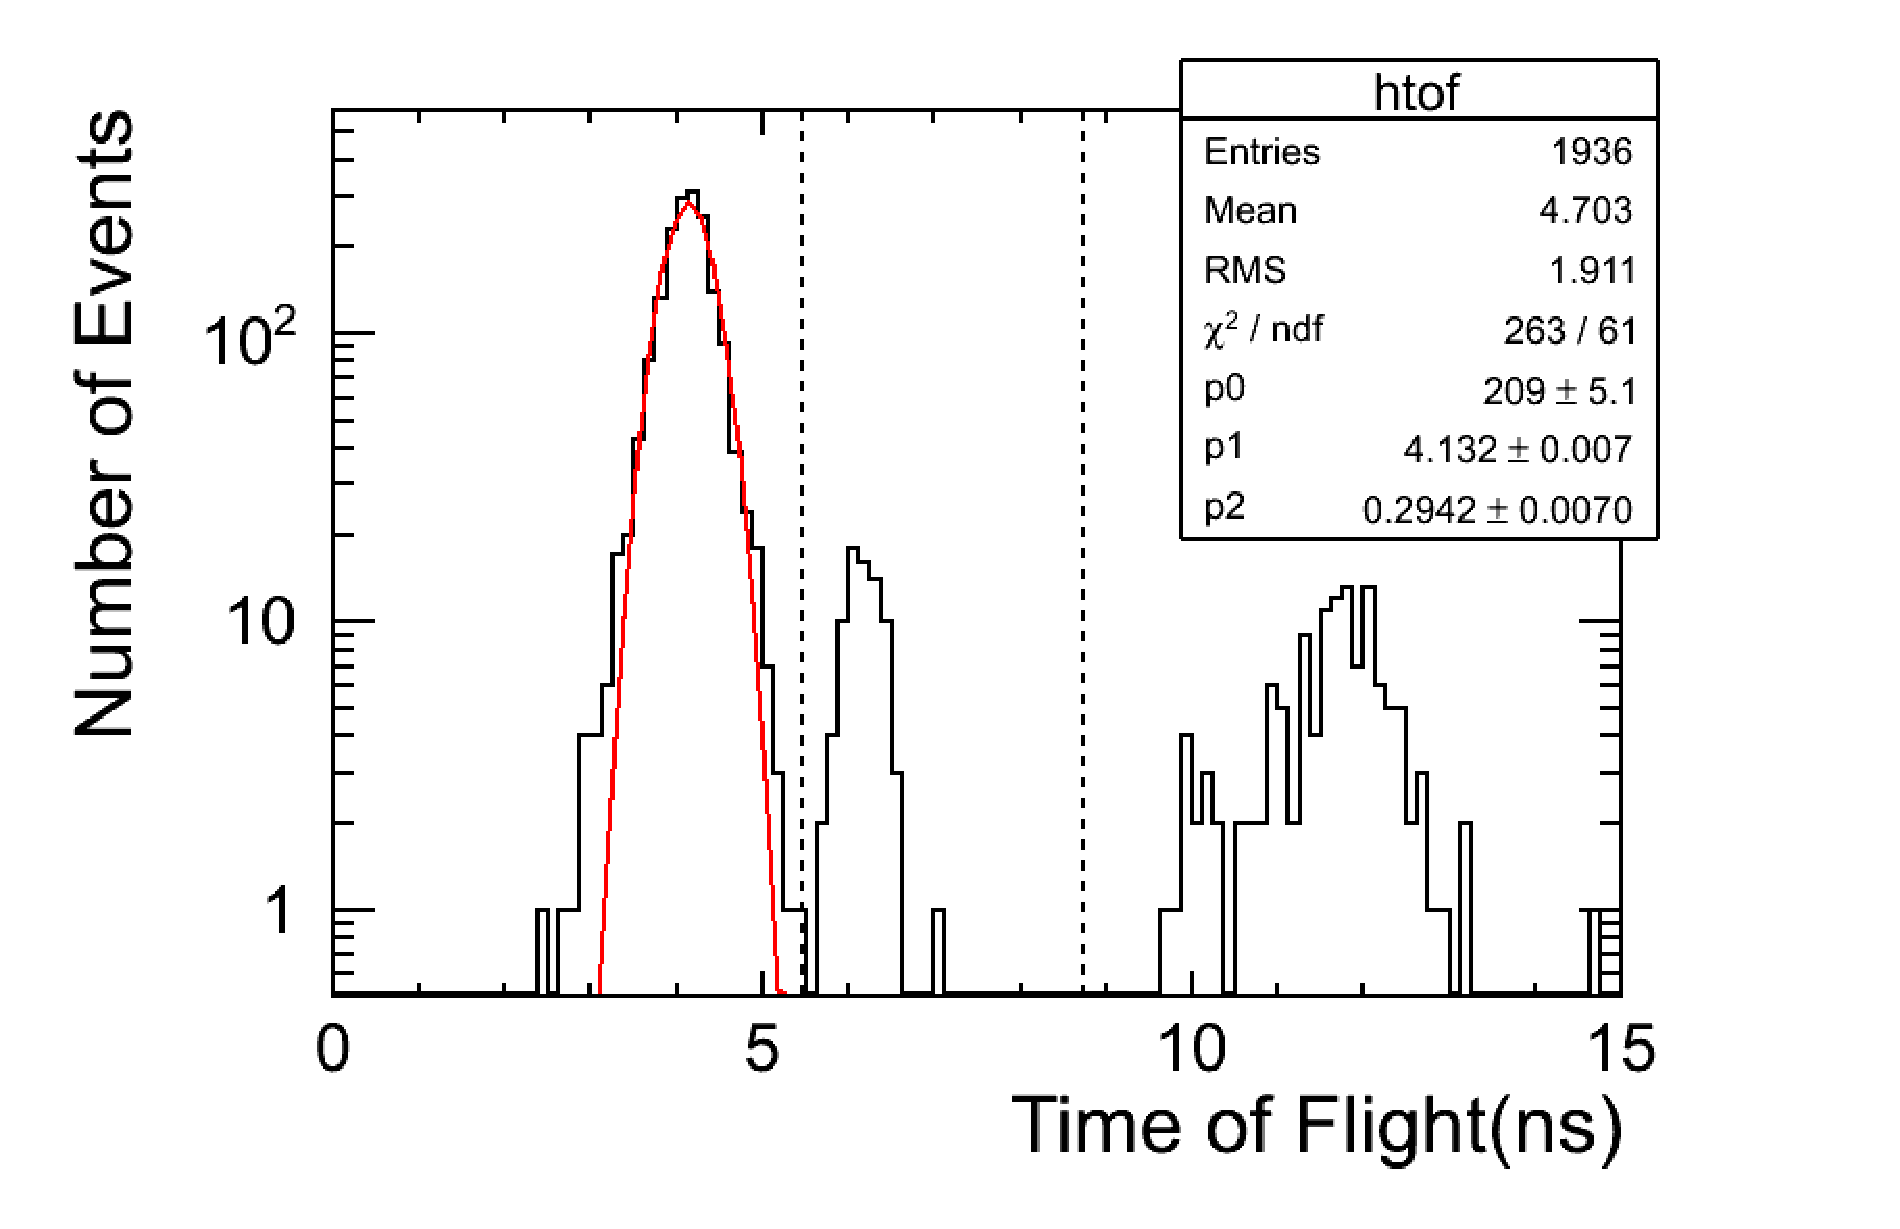
\includegraphics[width=10cm,clip]{fig/TOF.eps}
  \caption{TOF Counter}
  \label{fig:TOF}
\end{figure}

$K^{+}$ can selected very efficiently with Fitch Cherenkov Counter,
so we require the condition FC Signal($K$) is more than 2000
to get $K^{+}$ events in taking data.
Figure\ref{fig:TOF_cut} shows responce of the TOF Counters before and after above cut.
The histgram which filled with black is what is after cut.
This figure shows we can get high-purity $K^{+}$ samples with this condition.

\begin{figure}[htbp]
  \centering
  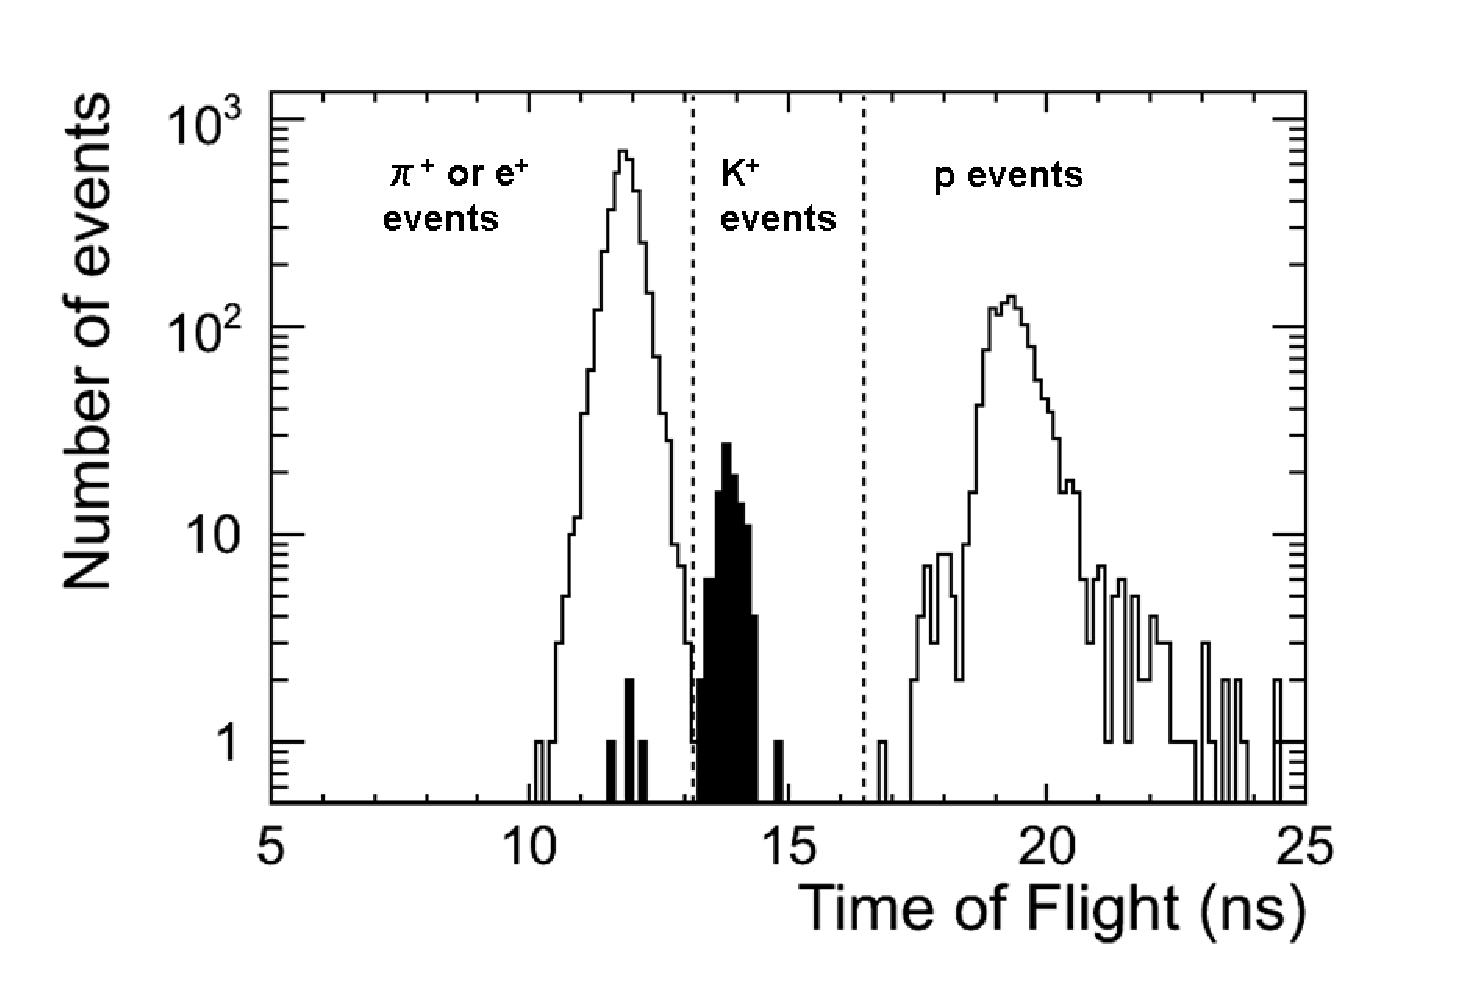
\includegraphics[width=10cm,clip]{fig/TOF_cut.eps}
  \caption{TOF Counter after $K^{+}$ selection}
  \label{fig:TOF_cut}
\end{figure}

Particles which satisfy all conditions for the same candidate are identified themselves, and the others are defined `uncertain` particles.
Herewith, we can identify beam particles with high purity before injection to 250L detector.
Table\ref{tb:component} shows the beam components of the data used for analysis.\\

\begin{table}
  \centering
  \begin{tabular}[htb]{ccccccc}\hline
    Run Number    & $e^{+}$ & $\pi^{+}$ & $K^{+}$ & $p$   & $uncertain$ & Number of Events \\ \hline
    42            & 68      & 1617      & 27      & 232   & 5           & 1949             \\
    48            & 128     & 1594      & 78      & 126   & 11          & 1937             \\
    49            & 0       & 341       & 0       & 1146  & 12          & 1499             \\
    52            & 0       & 0         & 3169    & 0     & 34          & 3203             \\
    55            & 0       & 0         & 8534    & 0     & 66          & 8600             \\
    59            & 0       & 0         & 5900    & 0     & 50          & 5950             \\
    60            & 0       & 0         & 1899    & 0     & 13          & 1912             \\ \hline
  \end{tabular}
  \label{tb:component}
  \caption{Beam components of data ued for analysis}
\end{table}

Run 52,55,59 and 60 are the data required the condition FC Signal($K$) is more than 2000 in taking data to get $K^{+}$ events.
Therefore the selection of $K^{+}$ on the analysis required by only TOF, that is, time of flight is 12.72$\sim$17.72ns, and the others are defined $uncertain$.
As table\ref{tb:component} shows, these data is almost occupied $K^{+}$ events and the ratio is $\sim$99.2\% on average.
